%%--------------------------------------------------
\subsection{Financial Market Simulation}
\label{ss:Market Simulation}
%% - - - - - - - - - - - - - - - - - - - - - - - - -

We developed the platform software Plham (Platform for Large-scale and
High-frequency Artificial Market), which can simulate financial
markets with thousands of stocks and hundreds of thousands of market
participants\cite{ToriiIzumiYamada2017}.  By joint research with Tokyo
Stock Exchange, the market simulation result using Plham supported a
new rule determination in the actual financial market.  Simulation
execution and management utilized the execution control system OACIS
developed in this project.  The information about the main part of
OACIS, improvement of a user interface, and the decision of
analysis/visualization application acquired by simulation execution
was fed back to the OACIS development team.  The result shown below
was obtained about the market simulation.

%%------------------------------
\subsubsection{Policy-making support of tick size reduction of Tokyo Stock Exchange}
%% - - - - - - - - - - - - - - -

About 100 kinds of parameter study were performed using the prototype
program of the small-scale financial market simulation in which 1,000
trading agents trade one kind of stocks
(\figref{fig:Figs.izumi/ticksize.eps})\cite{Mizuta2013a,doi:10.1002/isaf.1374,MizutaKosugiKusumotoMatsumotoIzumi2015}.
As compared with a simulation result and the actual data of Tokyo
Stock Exchange, the threshold of proper tick size (the minimum price
unit) was calculated from the fluctuation of a stock price.  This
simulation result was reflected in the plan of selection of the target
stocks in the tick size reduction of Tokyo Stock Exchange in 2014.
Furthermore, while developing an analytical theory which reproduces a
simulation result in good accuracy and helping an intuitive
understanding of the simulation result, the simulation model which
reduces a computational complexity was developed.

\begin{figure}[htb]
  \centering
  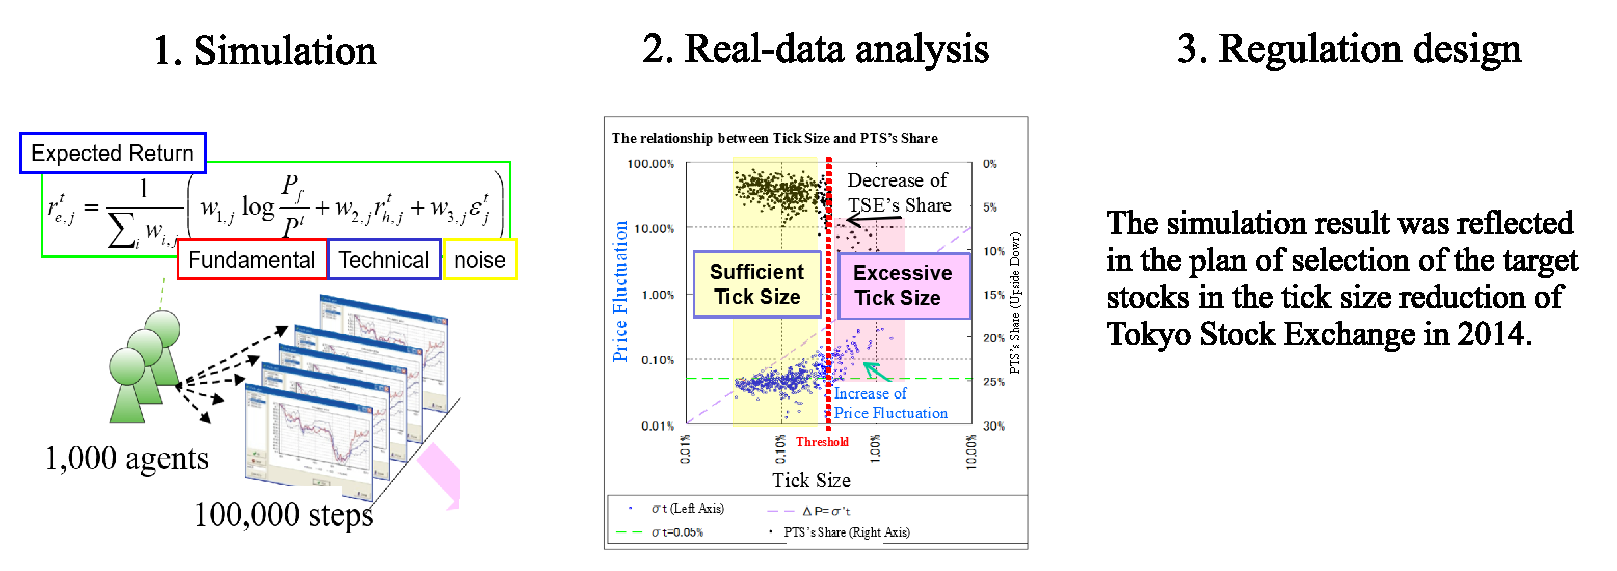
\includegraphics[width=.8\linewidth]{Figs.izumi/TickSize.eps}
  \caption{Impact analysis of the tick size reduction by a financial market simulation}
  \label{fig:Figs.izumi/ticksize.eps}
\end{figure}

%%------------------------------
\subsubsection{Simulation of Flash Crash}
%% - - - - - - - - - - - - - - -

The prototype model was extended using the parallel processing
language X10 to the larger-scale simulation which consists of 100
individual stocks and one index securities coupled to a stock price
average\cite{ToriiIzumiYamada2016}.  We investigated the conditions to
which the high-frequency arbitrage trading propagates a rapid price
change to other stocks using this model.  About 5000 kinds of
parameter sets were analyzed using social simulation management module
OACIS, and the combination of the trading strategies which a price
decline propagates to other stocks and the flash crash may occur was
specified (\figref{fig:Figs.izumi/hft.eps}).
We introduced the circuit
breaker into the model as a financial regulation which prevents such
fluctuation propagation and investigated the conditions where a
circuit breaker prevents propagation effectively, and the conditions
where it accelerated the propagation.

\begin{figure}[htb]
  \centering
  \includegraphics[width=.8\linewidth]{Figs.izumi/HFT.eps}
  \caption{Analysis of the price decline propagation by a simulation}
  \label{fig:Figs.izumi/hft.eps}
\end{figure}


%%------------------------------
\subsubsection{Analysis of the influence of risk management regulation}
%% - - - - - - - - - - - - - - -


By the joint research with a financial institution, we developed the
support method of the institutional design financial regulation such
as capital adequacy requirements\cite{YonenoIzumi2018}.  As a result,
the market became unstable when the market participants who manage a
market risk based on capital adequacy requirements increased in number
\figref{fig:Figs.izumi/var1.eps}).  An increase of the kind of
securities in which it trades showed that the instability by
regulation was eased (\figref{fig:Figs.izumi/var2.eps}).

\begin{figure}[htb]
  \centering
  \includegraphics[width=.8\linewidth]{Figs.izumi/VaR1.eps}
  \caption{The example of price fluctuation in having no capital adequacy requirements (left figure) and a simulation with regulation (right figure)}
  \label{fig:Figs.izumi/var1.eps}
\end{figure}

\begin{figure}[htb]
  \centering
  \includegraphics[width=.8\linewidth]{Figs.izumi/VaR2.eps}
  \caption{The ratio r of the agents imposed by regulation, and the relation between the number G of trading capital, and the instability (vertical axis) of a market}
  \label{fig:Figs.izumi/var2.eps}
\end{figure}


This artificial market simulation software Plham is released from
April 2016 (https://github.com/plham/plham).  Since it is
implementation by an agent model, it can reproduce the mixed
environment of various investment strategies seen in actual markets,
such as an HFT and an automatic transaction.  Since it is implemented
with the parallel processing language X10, it can run on various
scales from stand-alone PC to large-scale parallel execution
environment according to the scale of a simulation.  We are targeting
a researcher or not only an engineer but the financial working member,
and the policy maker as a user.

%\bibliography{ssecMarket}

%%++++++++++++++++++++++++++++++++++++++++++++++++++++++++++++++++++++++
% \begin{figure}
%   \centering
%   \includegraphics[width=.8\linewidth]{Figs.noda/figure-07.market_phase.eps}
%   \caption{Phase Diagram of Market Simulation}
%   \label{fig:Figs.noda/figure-07.market_phase.eps}
% \end{figure}
%%++++++++++++++++++++++++++++++++++++++++++++++++++++++++++++++++++++++



